\section{Brugere og opgaver}

De to vigtigste opgaver som prototypen skal understøtte er beskrevet i de
følgende afsnit.

\subsection{Oprettelse af medlemsskab}

Oprettelse af medlemsskab er en væsentlig del af Pensionistsagens hjemmeside.
Det er gennem dette medlemsskab at folk kan få attraktive rabatter og tilbud
på en lang række ting i hjemmesidens tilhørende webshop.

Idet en væsentlig del af hjemmesidens brugergruppe udgør personer med kun
ringe IT-kyndighed jf. PACT-analysen fra \cite{opgave2} er det vigtigt at
denne process er så simpel som muligt, samt at man let er i stand til at
finde tilmeldingssiden. Opgaven minder meget om scenariet ``Tilmelding til
Pensionistsagen'' fra \cite{opgave2} hvor Karl Koder hjælper et familiemedlem
med at tilmelde sig. Opgaven skal dog også være i stand til at blive løst
af en pensionist alene såfremt denne besider basale færdigheder om brug af
internettet.

Den kontekstuelle undersøgelse fra \cite{opgave3} gav ikke anledning til at
tilmeldingssiden skulle ændres i nogen væsentlig grad.

\subsubsection{Udførsel af opgaven}

Fra forsiden på Figur \ref{fig:opg1_trin1} klikker brugeren på
linket ``Medlemsservice'' i undermenuen hvorefter han får vist
skærmbilledet i Figur \ref{fig:opg1_trin2} og udfylder formularen som vist
i Figur \ref{fig:opg1_trin3}. Når brugeren har klikket på ``Fuldfør
tilmelding''-knappen bliver han mødt med en side der kort fortæller at
tilmeldingen lykkedes som i Figur \ref{fig:opg1_trin4}.

\begin{figure}[h]
    \centering
    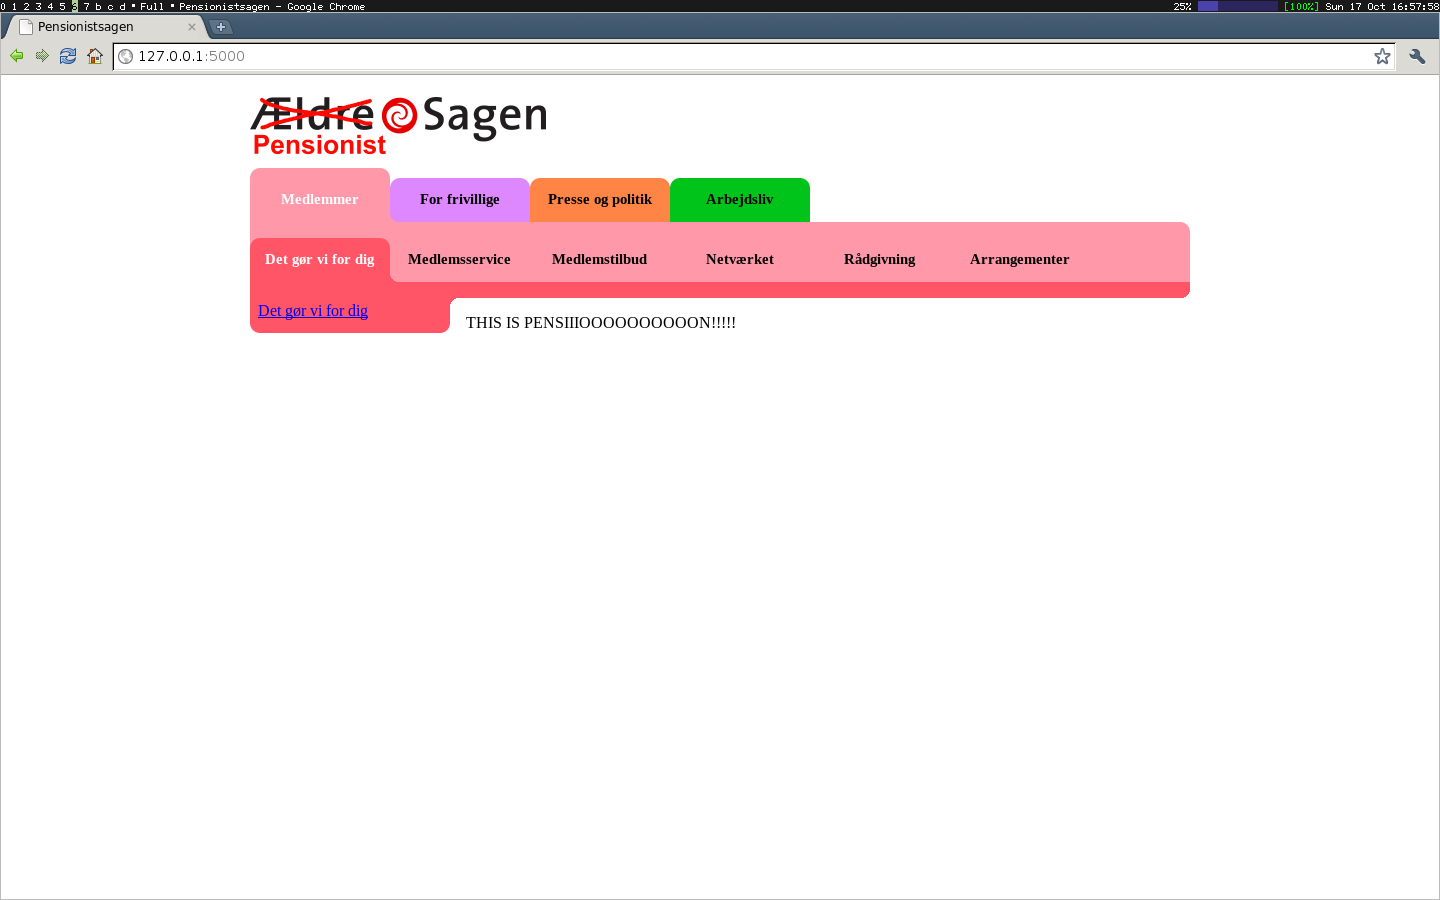
\includegraphics[width=.9\textwidth]{billeder/opgave1_trin1.png}
    \caption{Pensionistsagens forside. Indeholder i prototypen ikke nogen relevant information.}
    \label{fig:opg1_trin1}
\end{figure}
\begin{figure}[h]
    \centering
    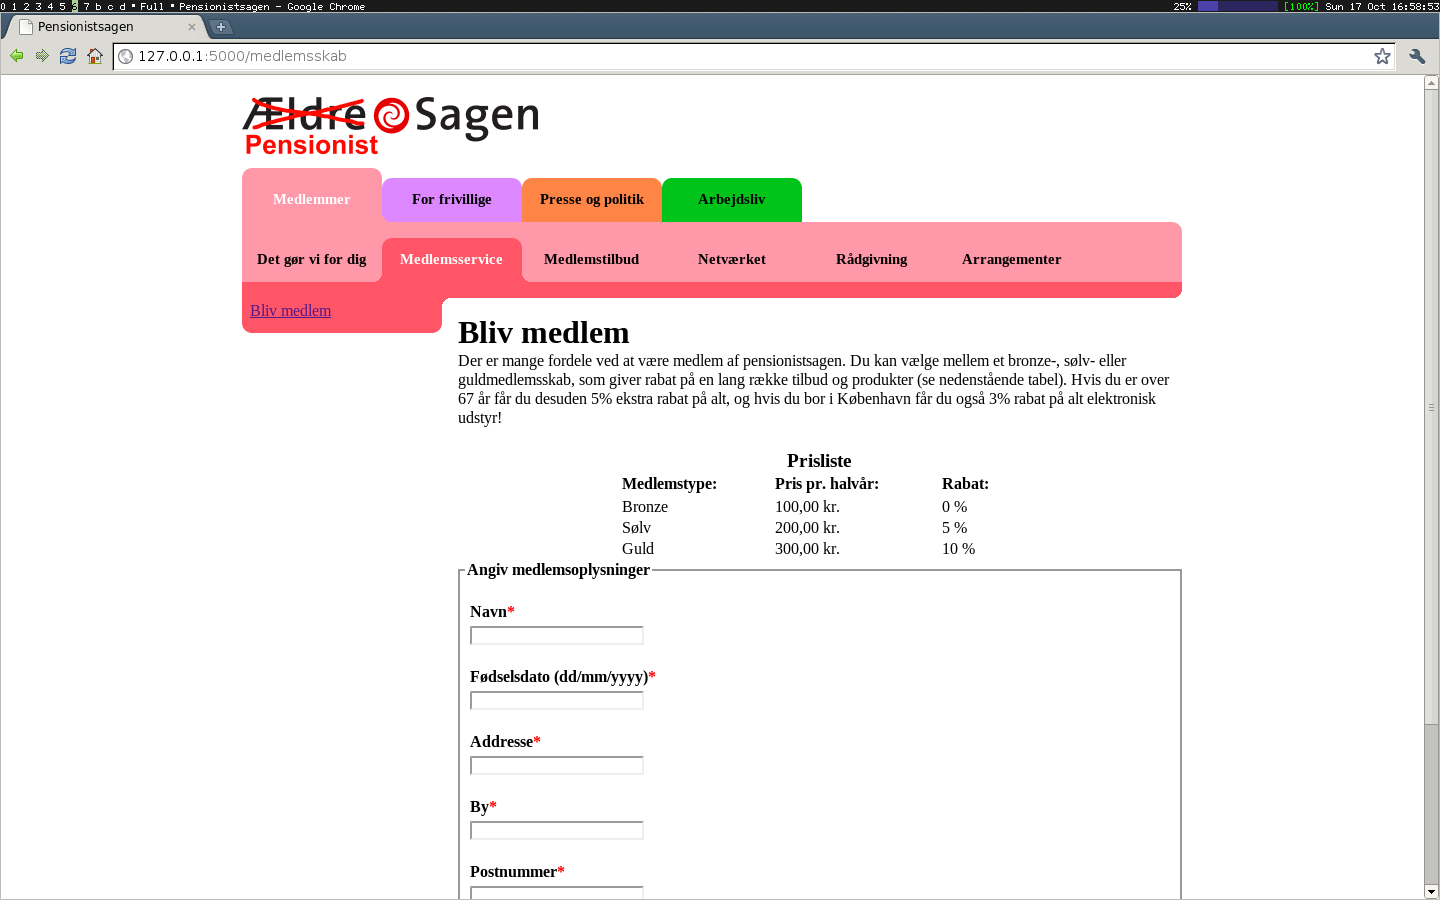
\includegraphics[width=.9\textwidth]{billeder/opgave1_trin2.png}
    \caption{Forsiden for ``Bliv medlem''. Brugeren kan her se en forklarende tekst om de forskellige medlemstyper, se en oversigt i tabellen samt udfylde personlige informationer.}
    \label{fig:opg1_trin2}
\end{figure}
\begin{figure}[h]
    \centering
    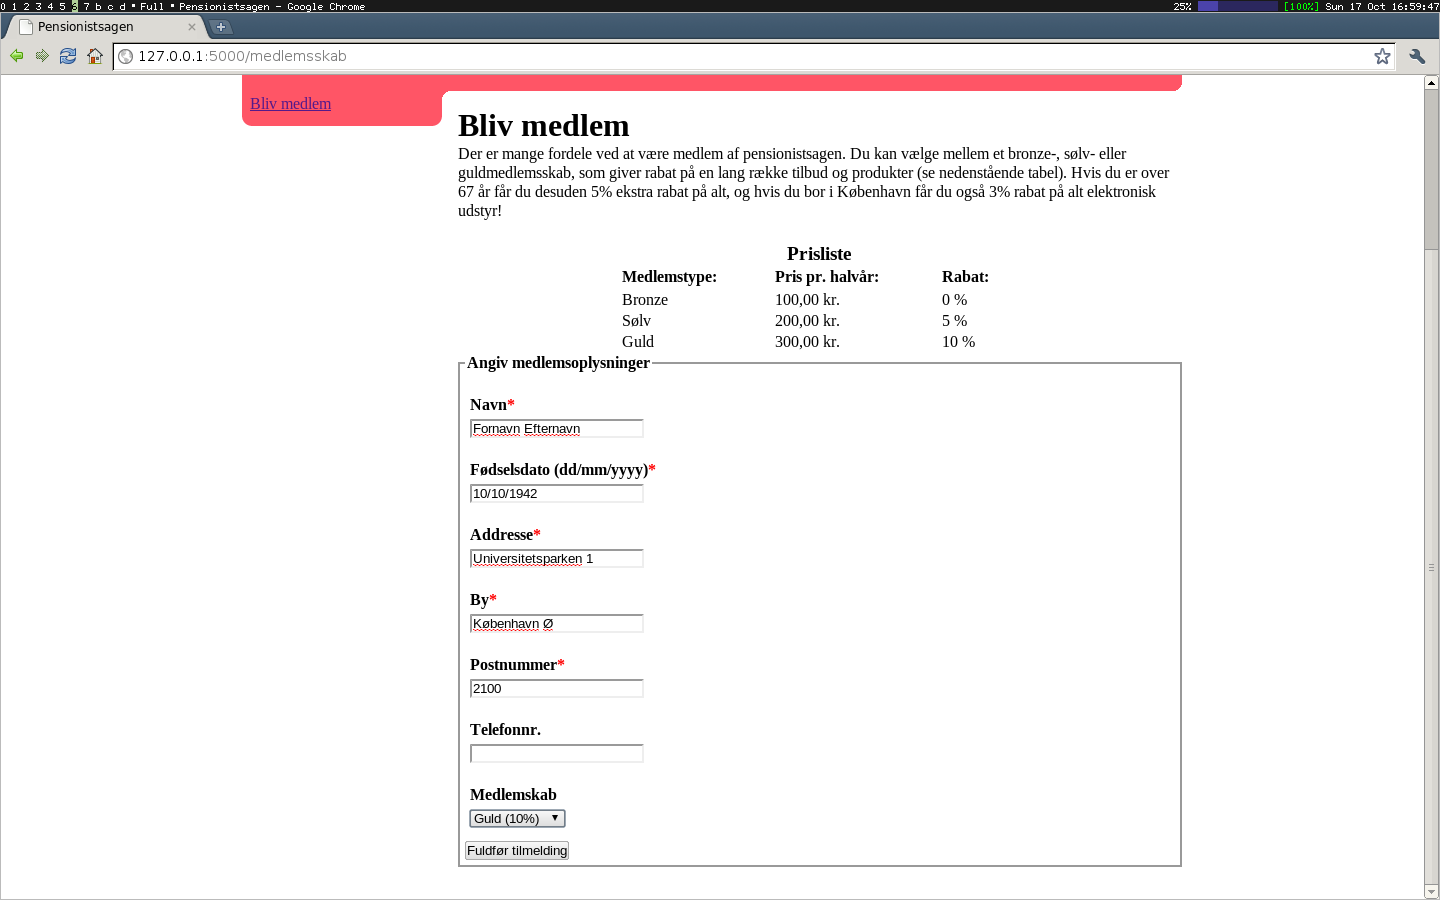
\includegraphics[width=.9\textwidth]{billeder/opgave1_trin3.png}
    \caption{Felterne i formularen er blevet udfyldt.}
    \label{fig:opg1_trin3}
\end{figure}
\begin{figure}[h]
    \centering
    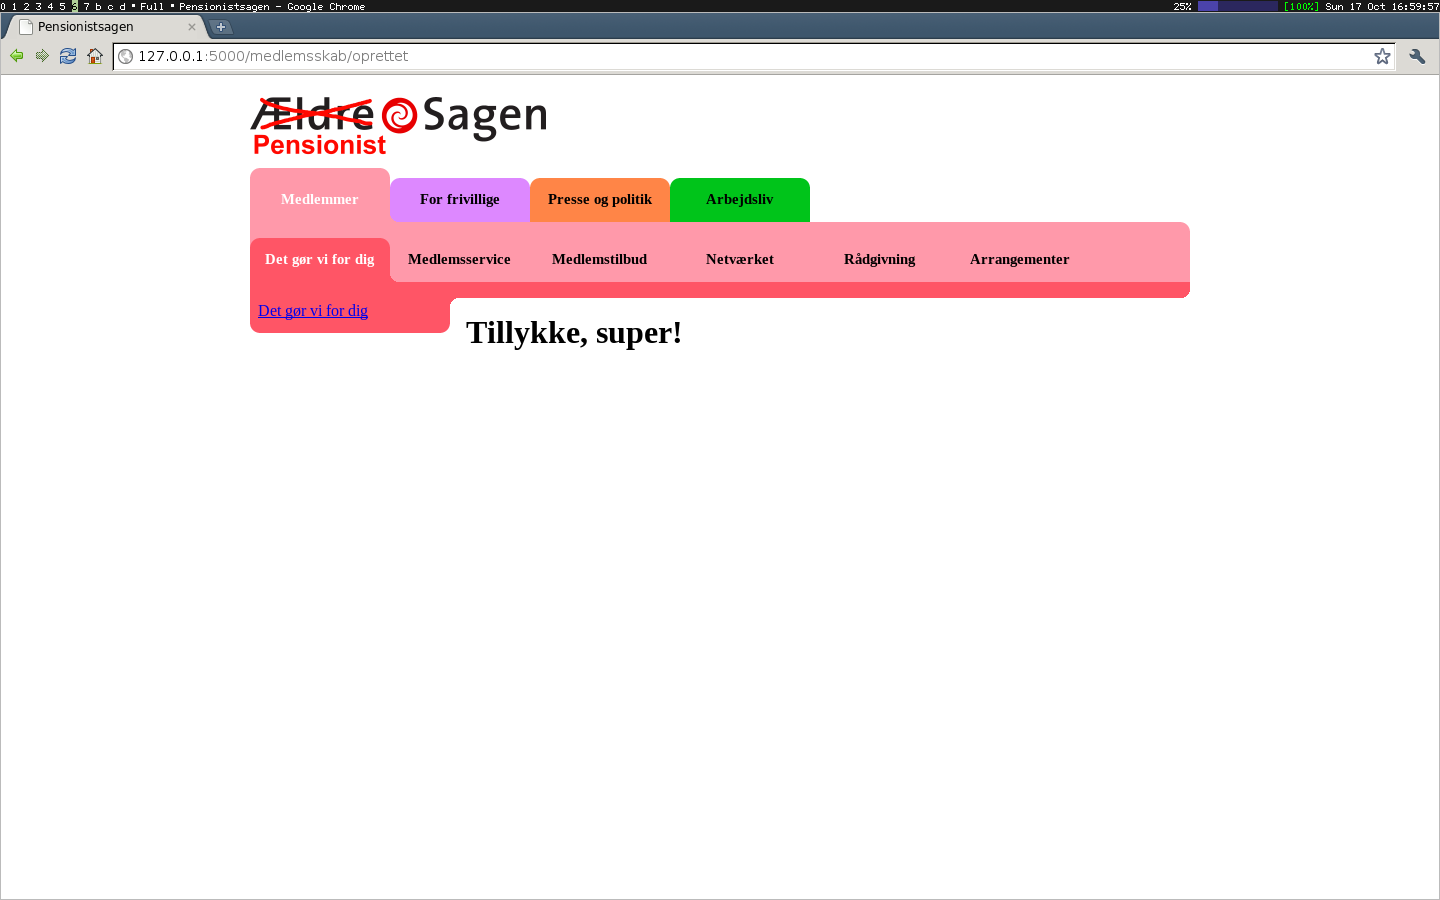
\includegraphics[width=.9\textwidth]{billeder/opgave1_trin4.png}
    \caption{Formularen er blevet udfyldt og sendt.}
    \label{fig:opg1_trin4}
\end{figure}

\subsection{Køb af tilbud/varer}


